\documentclass[10pt]{article}%{scrartcl} % Beginn der LaTeX-Datei
\usepackage[utf8]{inputenc}  % für Unix-Systeme
\usepackage{amsmath,amssymb,mathtools}  % erleichtert Mathe 
\usepackage{tabularx}
\usepackage{enumerate}% schicke Nummerierung
\usepackage{geometry}
\geometry{a4paper,left=30mm,right=30mm, top=3cm, bottom=2cm} 
\usepackage{graphicx} % für Grafik-Einbindung
%\usepackage[dvips]{hyperref}
\usepackage{mdwlist}
\usepackage[labelfont=bf]{caption}
\usepackage{subcaption}

\usepackage[ngerman]{babel}
\addto\captionsngerman{\renewcommand{\figurename}{Abb.}}
%\usepackage[T1]{fontenc}
%\usepackage{lmodern}
 % Einstellungen, wenn man deutsch schreiben will, z.B. Trennregeln
  % ermöglicht die direkte Eingabe von Umlauten und ß
  % evt. obige Zeile ersetzen durch
  % \usepackage[utf8]{inputenc}
  % \usepackage[ansinew]{inputenc}  % für Windows
  % \usepackage[applemac]{inputenc} % für den Mac

%%%%%%%%%%%%%%%%%%%%%%%%%%%%%%%%%%%%%%%%%%%%%%%%%%%%%%%%%%%%%%%%%%
%
%  ntheorem
%
\usepackage[thmmarks,amsmath,hyperref,noconfig]{ntheorem} 
  % erlaubt es, Sätze, Definitionen etc. einfach durchzunummerieren.
\newtheorem{satz}{Satz}[section] % Nummerierung nach Abschnitten
\newtheorem{hilfssatz}[satz]{Hilfssatz}
\newtheorem{kor}[satz]{Korollar}

\theorembodyfont{\upshape}
\newtheorem{beispiel}[satz]{Beispiel}
\newtheorem{bemerkung}[satz]{Bemerkung}
\newtheorem{definition}[satz]{Definition}

\theoremstyle{nonumberplain}
\theoremheaderfont{\itshape}
\theorembodyfont{\normalfont}
\theoremseparator{.}
\theoremsymbol{\ensuremath{_\blacksquare}}
\newtheorem{beweis}{Beweis}
\qedsymbol{\ensuremath{_\blacksquare}}
%\theoremclass{LaTeX}
%
% Ende ntheorem
%
%%%%%%%%%%%%%%%%%%%%%%%%%%%%%%%%%%%%%%%%%%%%%%%%%%%%%%%%%%%%%%%%%%

%\pagestyle{empty}
%
% Ändern der bedruckten Fläche der Seite
% \addtolength{\textwidth}{3cm}  % Befehl mit zwei Argumenten
% \addtolength{\textheight}{3cm}
% \hoffset-2cm % verschiebt das Textfenster nach links
% \voffset-5mm % verschiebt das Textfenster nach oben
%
%\parindent=0pt %% keine Einzug zu Beginn von Abs\"atzen
%\parskip=2mm   %% erzeugt einen zusätzliche Zeilenabstand zwischen
                %% Absätzen. Nötig bei \parindent=0pt


\usepackage{pgf}
\usepackage{tikz}
\usetikzlibrary{arrows,automata,calc,patterns,positioning,shapes}


%%%%%%%%%%%%%%%%%%%%%%%%%%%%%%%%%%%%%%%%%%%%%%%%%%%%%%%%%%%%%%%%%%
%
%  ermöglicht, farbigen Text zu drucken.
%
\usepackage{color}
% Und nun werden die Farben definiert - daran können Sie nach Belieben selber rumspielen.
\definecolor{white}{rgb}{1,1,1}
\definecolor{darkred}{rgb}{0.3,0,0}
\definecolor{darkgreen}{rgb}{0,0.3,0}
\definecolor{darkblue}{rgb}{0,0,0.3}
\definecolor{pink}{rgb}{0.78,0.09,0.51}
\definecolor{purple}{rgb}{0.28,0.24,0.55}
\definecolor{orange}{rgb}{1,0.6,0.0}
\definecolor{grey}{rgb}{0.4,0.4,0.4}
\definecolor{aquamarine}{rgb}{0.4,0.8,0.65}


\DeclareMathOperator{\GL}{GL} % einige Macro, siehe am Ende Abschn. 2
\newcommand{\N}{\mathbb{N}}
\newcommand{\Z}{\mathbb{Z}}
\newcommand{\Q}{\mathbb{Q}}
\newcommand{\R}{\mathbb{R}}
\newcommand{\PP}{\mathbb{P}}
\newcommand{\PPX}{\mathbb{P}^X}
\newcommand{\C}{\mathbb{C}}
\newcommand{\cP}{{\mathcal P}} 

\setlength{\parindent}{0cm}
\setlength{\parskip}{.2cm}
\setlength{\fboxsep}{0pt}
%\setlength{\fboxrule}{.2mm}

%\usepackage{showframe}

\begin{document}

\author{Gruppe 04 -- Alex Oks, Markus Görlich, Simon Stieber}
\title{Selbstorganisierende, adaptive Systeme - Blatt 03}
%\date{} %hier können Sie ein Datum eingeben, auch leer, sonst wird es
         %automatisch erzeugt

\maketitle % erzeugt den Kopf
%%\let\clearpage\relax
\section{Aufgabe 1}
\subsection{b}
Erwartung: Bei ausreichender Startenergie reicht dennoch ein einzelner Zombie aus um alle zu infizieren, jedoch sterben die Zombies logischerweise, wenn keine Menschen mehr übrig sind (Erwartung bestätigt)

\section{Aufgabe 2}
\subsection{a)}
Siehe Code
\subsection{b)}
\subsubsection{1. Versuch: Mittelgroße Welt und mittlere Anzahl an Bohnen}
Bei mittleren Einstellungen für Bohnenanzahl und Weltgröße steigt die Entropie stetig gegen die Maximalentropie an, erreicht diese jedoch nie. \\
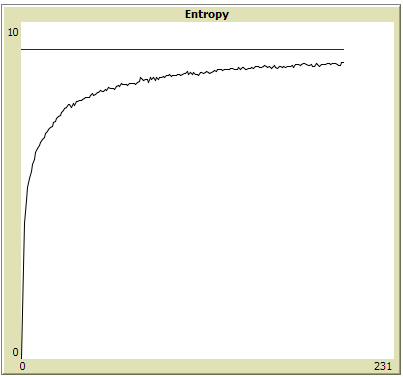
\includegraphics [scale = 0.85]{2-mittel.png}
\subsubsection{2. Versuch: Weltgröße und Bohnenanzahl erhöhen}
Bei hohen Einstellungen für Bohnenanzahl und Weltgröße steigt die Entropie auch stetig, aber langsamer an. \\
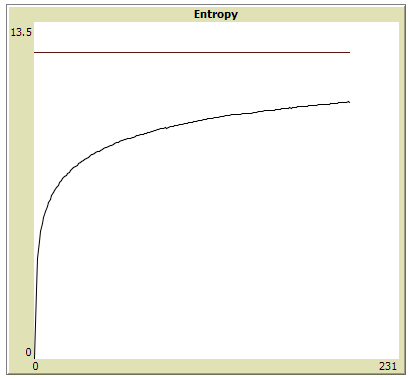
\includegraphics [scale = 0.85]{2-hoch.png}
\subsubsection{3. Versuch: Bohnenanzahl größer als Patch-Anzahl}
Wenn man die Anzahl der Bohnen so erhöht, dass es mehr Bohnen als Felder gibt,
steigt die Entropie auf einen Wert weit unter der Maximalentropie an und pendelt dort ein. Das liegt daran, dass in diesem Szenario immer mehrere Bohnen auf einem Feld landen und es somit sehr unwahrscheinlich bzw. unmöglich ist, dass die Bohnen gleich verteilt sind. \\
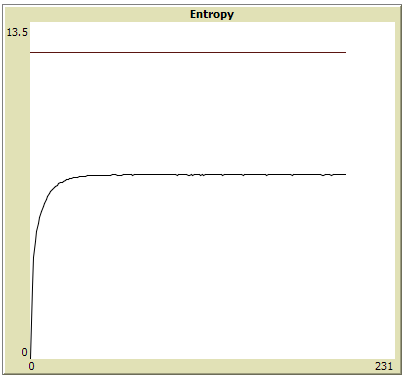
\includegraphics [scale = 0.85]{2-vieleBohnen.png}
\section{Aufgabe 3}
Staubsaugerroboter:
\subsection{a)}
Der simple Staubsaugerroboter verhält sich unter den getroffenen Annahmen in Folie 16
rational. Zeigen Sie dies.

Rationalität:
"Ein Agent agiert rational, wenn er unter Berücksichtigung all seines
eingebauten und erworbenen Wissens über die Umwelt für alle
Wahrnehmungssequenzen diejenige Aktion wählt, die den erwarteten
Wert des Performancemaß maximiert." Folie 16

\begin{itemize}
	\item eingebautes und erworbenes Wissen
	\item für alle Wahrnehmungssequenzen
	\item Wahl der Aktion die den erwarteten Wert der Performance maximiert
\end{itemize}

Hier: P ist gegeben: Zahl d sauberen Zellen nach n Schritten.
Wahrnehmung: Nur zwei Zellen in der Nachbarschaft und die fixe Geographie.
Nun müssen die Aktionen so gewählt werden, das P maximal wird.
Dann ist der Agent rational.

\subsection{b)}
Nehmen wir nun an, unnötige Bewegung würde bestraft, da zusätzliche Energie verbraucht
wird. Beschreiben Sie zunächst ein geeignetes Performancemaß P sowie eine Agentenfunk-
tion f , welche rational agiert. Beschreiben Sie, warum der simple Agent nun nicht mehr
rational ist.

Überlegungen:
Lieber nicht bewegen als zu viel bewegen.
Fahrt über bereits geputzte Zelle wird bestraft.
P':
P ist festgelegt als die Anzahl sauberer Zellen über den Zeitraum von T=100 Schritten. (P alt)
Für jeden unnötigen Schritt werden Punkte abgezogen (Strafpunkte).

$f: P' => A$
Schritte in bereits geputzte Zellen sollen tunlichst vermieden werden.

Der Agent ist nicht mehr rational, weil die Wahl der Aktion jetzt nicht mehr nur von seinem Wissen abhängt sondern auch von einer möglichen Strafe.

\subsection{c)}
Geben Sie eine PEAS-Beschreibung und Kategorisierung anhand der vorgestellten Dimensionen für die folgenden Task-Umgebungen an:
\begin{enumerate}
	\item Bieten auf einen Gegenstand bei einer Auktion
	\item Suche nach Wrackteilen mit autonomen Unterwasser-Fahrzeugen
	\item Intelligenter Stromverbrauch: Zu Zeiten hoher Strompreise sollten geplante energieintensive Vorgänge verschoben werden
\end{enumerate}

\begin{table}
	\centering
	\begin{tabular}{p{0.5cm}|p{3cm}|p{3cm}|p{3cm}|p{3cm}}
		Task  &	Performance & Environment & Actuators & Sensors \\
		\hline
		1 & Erhalt des Gegenstandes, Niedriger Preis & Auktion(On-/Offline), andere Bieter, (Auktionsrausch) & Hand zum bieten & Visuell: Wie ändert sich der Preis, was machen die Anderen \\
		\hline
		2 & Gefundene Wrackteile, Verbrauchte Energie & Gesteine, Meer, andere Schiffe, Tiere, Mensch, Botanik & Propeller, Steuer, Motor & Kompass, Tiefensensor, Sonar, Radar, IMU, Drucksensor \\
		\hline
		3 & Kosten für Vorgang-> Reduktion & Strommarkt, andere Wettbewerber, Tag und Nacht Rhythmus des Strompreises & Vorgang nicht starten oder starten oder unterbrechen (falls möglich) & Visuell: Beobachtung des Strompreises am Markt \\
	\end{tabular}
	\caption{PEAS Analyse}
\end{table}

\subsection{d)}
Entwickeln Sie eine Zustandsmaschine für den Staubsaugerroboter aus der Vorlesung (Folie
36). Der Roboter soll periodisch alle Felder besuchen und Schmutz möglichst effizient entfernen. Kann Nichtdeterminismus hilfreich sein? Geben Sie den Wert der Agentenfunktion
für ein paar Wahrnehmungssequenzen an.

Nichtdeterministisch: Dreck finden und putzen:

\begin{tikzpicture}[->,>=stealth',shorten >=1pt,auto,node distance=5cm,
semithick]
\tikzstyle{every state}=[fill=red,draw=none,text=white]

\node[initial,state] (clean)                    {$cell: clean$};
\node[state]         (dirty) [right of=clean] {$cell: dirty$};

\path (clean) edge [bend left]             node {dirty cell in sight / move to dirty cell} (dirty)
(dirty) edge [bend left]				node {clean the cell / cell cleaned} (clean);
\end{tikzpicture}

Kann hilfreich sein wenn immer nur ein Teil des Raumes verschmutzt wird und der Rest sauber bleibt.

Periodisch:

\begin{tikzpicture}[->,>=stealth',shorten >=1pt,auto,node distance=8cm,
semithick]
\tikzstyle{every state}=[fill=red,draw=none,text=white]

\node[initial,state, align=left] (clean)                    {$cell: clean$,\\ $Coordinates:X, Y$};
\node[state, align=left]         (a) [right of=clean] {$cell: dirty$\\ $Coordinates:X+1, Y$};
\node[state, align=left]         (b) [below of=clean] {$cell: clean$\\ $Coordinates:X+2, Y$};
\node[state, align=left]         (c) [below of=a] {$cell: dirty$\\ $Coordinates:X+2, Y+1$};
\node[state, align=left]         (d) [below of=b] {...};

\path (clean) edge           node {move to next cell} (a)
(a) edge [loop above]				node {clean the cell / cell cleaned} (b)
(a) edge           node {move to next cell} (b)
%(b) edge [loop above]				node {clean the cell / cell cleaned} (c)
(c) edge [loop above]				node {clean the cell / cell cleaned} (d)
(b) edge           node {move to next cell} (c)
(d) edge [loop above]				node {clean the cell / cell cleaned} (clean)
(c) edge           node {move to next cell} (d);

\end{tikzpicture}

Wie man sieht hat man hier Probleme einen EA zu finden, da es eine große Anzahl Stati gibt, abgeleitet von den Koordinaten.

Agentenfunktion: Ausgabe: Performance gut bei clean, schlecht bei betreten einer sauberen Zelle.

\subsection{e)}
Wahrnehmungsmenge:
Wahrnehmung über Kameras: Rotes Licht beim vorderen Auto.
Wahrnehmungsfolge:
Annahme: Blinker sind max. 0,7 Sekunden an.
\begin{itemize} 
	\item Kamera mit 24 FPS
	\item Blinker dauert max. ca. 0,7 Sekunden an, abhängig v. Hersteller und evtl. Modell
	\item Nach $24 * 0,7 = 16,8$ also 17 Frames dauerhaft rot im Bremslicht muss gebremst werden
\end{itemize}
Agentenfunktion:

\begin{tikzpicture}[->,>=stealth',shorten >=1pt,auto,node distance=5cm,
semithick]
\tikzstyle{every state}=[fill=red,draw=none,text=white]

\node[initial,state] (clean)                    {red light in sight};
\node[state]         (dirty) [below of=clean] {no red light in sight};
\node[state]         (wait) [right of=clean] {wait - count time};

\path (wait) edge [bend left]             node {aborted - indicator/do not break} (dirty)
(wait) edge [bend left]             node {time passed - no indicator/break} (clean)
(clean) edge [bend left]				node {wait 17 frames} (wait)
(dirty) edge [bend left]				node {see red light} (clean);
\end{tikzpicture}

\end{document}